Máy co góc plasma (\textit{Angular pinch}) sử dụng từ trường để tăng tốc và định hướng dòng plasma, do đó nó có thể tạo ra một vụ nổ plasma tại một mục tiêu ngay lập tức. Thiết bị được thể hiện trên hình dưới. Có một tấm dẫn xung quanh ống thủy tinh chân không và chứa một thanh mục tiêu có cùng chiều dài, bỏ qua độ dày của thành ống thủy tinh và độ dày của vỏ ruột dẫn, và $ H \gg R_{ 2} $. Ống chứa đầy hiđro bị ion hóa thành plasma có mật độ số điện tích dương và âm đều là $n$. Khi $ t = 0 $, người ta đặt một nguồn điện vào vỏ dây dẫn để dòng điện tăng nhanh từ 0 đến $ I $ và dòng điện $ I $ được giữ nguyên trong một khoảng thời gian, dòng điện chạy đều dọc theo hướng tiếp tuyến của vỏ hình trụ. Bỏ qua chuyển động nhiệt của các hạt, tương tác Coulomb và va chạm giữa các hạt, điện tích nguyên tố là $ e $, khối lượng của các electron và hạt nhân hydro lần lượt là $ m_{e}, m_{p} $.

\begin{figure}[!htb]
    \centering
    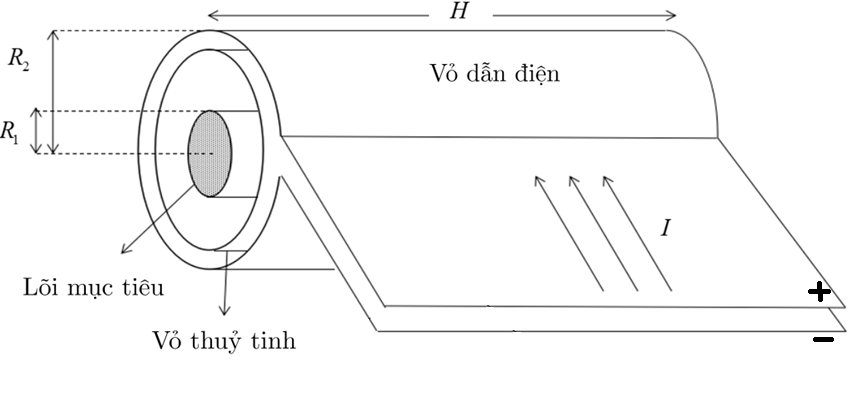
\includegraphics[scale=0.55]{Problem_8/P8.png}
    \label{fig_P8}
\end{figure}
\begin{enumerate}[label=\textbf{\alph*,}]\itemsep0em
\item Một hạt có điện tích $ q $ và khối lượng $ m $ ở khoảng cách từ trục trung tâm $ r \left (R_{1} <r <R_{2} \right) $ sau khi dòng điện ổn định tới $ I $. Tìm tốc độ tức thời $ v_{0} $ của hạt.    
    \item Tìm thời điểm $ t (r) $ khi hạt trong câu hỏi trước chuyển động đến vị trí $ R_{1} $.
    \item Giả sử hạt va chạm với thanh mục tiêu hoàn toàn không đàn hồi, tìm áp suất $ P (t) $ trên bề mặt của thanh mục tiêu tại thời điểm $ t $. Trên thực tế, plasma trong ống là các electron và hạt nhân hydro bị ion hóa, điều này cho thấy chuyển động của một loại hạt có thể bị bỏ qua khi $ t $ nhỏ, và ảnh hưởng của hạt này cần được bỏ qua trong câu trả lời cuối cùng.
    \item Xác định thông số thiết bị $ \beta = \cfrac {P_{\max}} {\omega_{B}} $, trong đó $ \omega_{B} $ là mật độ năng lượng của từ trường chân không và độ lớn của nó là $ \cfrac {B^{2}} {2 \mu_{0}} $. Sau đó, so sánh nó với $ \beta \left(\approx 10^{-1} \sim 1 \right) $ của hầu hết các thiết bị Tokamak (định hướng dòng plasma dạng donut) và thể hiện những ưu điểm của máy co góc. Đối với phép tính số trong câu hỏi này, hãy thay $\cfrac{\mu_{0}}{4 \pi} = 1 \times 10^{- 7} \mathrm {~N} / \mathrm {A}^{2}$, $H = 30.0 \mathrm {~m}$, $R_{1} = 1.0 \mathrm{~mm}$, $R_{2} = 1.00 \mathrm{~m}$, $n = 1.00 \times 10^{8} \mathrm {~m}^{-3}$.
\end{enumerate}

\begin{flushright}
    (Biên soạn bởi Zinc và Yukon)
\end{flushright}